% Graphic: Analise de épocas de treinamento no Experimento Delta
% \begin{figure*}[!ht]
\begin{figure}[H]
\centering
	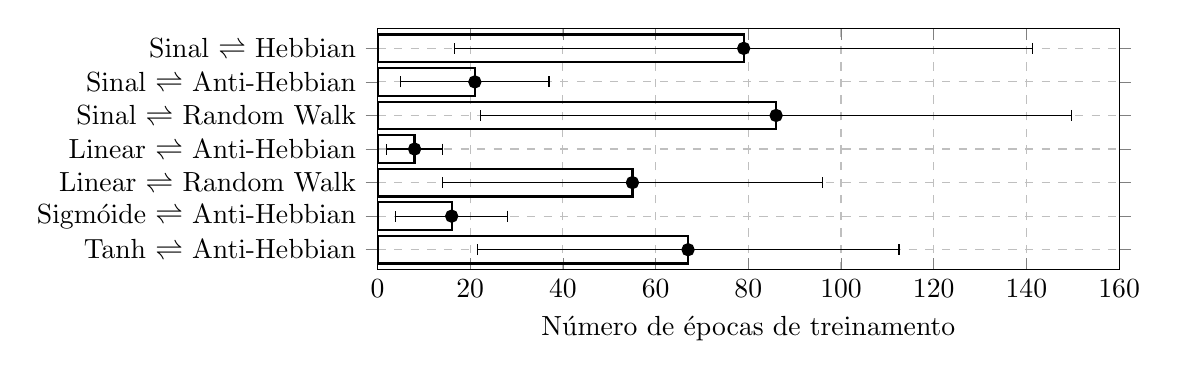
\begin{tikzpicture}
		\begin{axis}[
			%title={Número médio de épocas de treinamento com desvio padrão no Experimento $\delta$},
			symbolic y coords={Tanh $\rightleftharpoons$ Anti-Hebbian, Sigmóide $\rightleftharpoons$ Anti-Hebbian, Linear $\rightleftharpoons$ Random Walk, Linear $\rightleftharpoons$ Anti-Hebbian, Sinal $\rightleftharpoons$ Random Walk, Sinal $\rightleftharpoons$ Anti-Hebbian, Sinal $\rightleftharpoons$ Hebbian},
			xbar,
			xmin=0,
			xlabel={Número de épocas de treinamento},
			bar width=10pt,
			ytick=data,
			legend pos=north east,
			ymajorgrids=true,
			xmajorgrids=true,
			grid style=dashed,
			height=4.65cm,
			width=11cm,
			xmin=0, xmax=160,
			%nodes near coords, nodes near coords align={horizontal},
		]
		 
		\addplot[color=black, solid, thick, mark=*] plot[error bars/.cd, x dir=both, x explicit]
			coordinates {
				(79,Sinal $\rightleftharpoons$ Hebbian) +- (62.4,95.6)
				(21,Sinal $\rightleftharpoons$ Anti-Hebbian) +- (16,26)
				(86,Sinal $\rightleftharpoons$ Random Walk) +- (63.8,108.2)
				(8,Linear $\rightleftharpoons$ Anti-Hebbian) +- (6.1,9.9)
				(55,Linear $\rightleftharpoons$ Random Walk) +- (41,69)
				(16,Sigmóide $\rightleftharpoons$ Anti-Hebbian) +- (12.1,19.9)
				(67,Tanh $\rightleftharpoons$ Anti-Hebbian) +- (45.5,88.5)
			}; %\legend{Número médio de épocas}
		 
		\end{axis}
	\end{tikzpicture}
	\caption{Número médio de épocas com desvio padrão.}
	\label{graph:epochsResultsDelta}
\end{figure}